\documentclass[letterpaper, 10 pt, conference]{ieeeconf}  % Comment this line out
                                                          % if you need a4paper
%\documentclass[a4paper, 10pt, conference]{ieeeconf}      % Use this line for a4
                                                          % paper

\IEEEoverridecommandlockouts                              % This command is only
                                                          % needed if you want to
                                                          % use the \thanks command
\overrideIEEEmargins

\usepackage{graphicx}
\usepackage{lipsum}  
\usepackage{xcolor}
\usepackage{titlesec}
\usepackage{hyperref}
\hypersetup{
    colorlinks=true,
    linkcolor=blue,
    filecolor=magenta,      
    urlcolor=cyan,
    pdftitle={Overleaf Example},
    pdfpagemode=FullScreen,
    }
\PassOptionsToPackage{unicode}{hyperref}
\PassOptionsToPackage{naturalnames}{hyperref}

\titleformat{\subsection}
{\color{blue}\normalfont\itshape}
{\color{blue}\thesubsection}{1em}{}

\newcommand{\subtitle}[1]{{\\ \small \normalfont \color{purple} #1}}


\graphicspath{ {images/} }

\title{\LARGE \bf
JUSTFAIR \\{\color{blue}Datasheet}
}

\begin{document}


\maketitle
\thispagestyle{empty}
\pagestyle{empty}

%%%%%%%%%%%%%%%%%%%%%%%%%%%%%%%%%%%%%%%%%%%%%%%%%%%%%%%%%%%%%%%%%%%%%%%%%%%%%%%%
\section{Motivation}

\subsection{For what purpose was the dataset created?}

This dataset was created to increase the ease of access to data on public criminal trials. Specifically, it combines information from the US sentencing commission, Federal judicial center, PACER, wikipedia, and Federal Judicial Center biographies to create a dataset of defendants and their demographic characteristics with information about their crimes, their sentences, and the identity of the sentencing judge \cite{ciocanel2020justfair}.

\subsection{Who created the dataset? \subtitle{Is it an official law enforcement or government body? An academic research team? Other?}}

The dataset was created by researchers at the Institute for the Quantitative Study of Inclusion, Diversity, and Equity (QSIDE): Maria-Veronica Ciocanel, Chad Topaz, Rebecca Santorella, Shilad Sen, Christian Smith, and Adam Hufstetler.

\subsection{Was there a specific task in mind, or gap that needed to be filled?}

The authors wished to determine whether judges with significant sentencing outcome disparities across the race of defendants were due to racial bias by creating a dataset with sufficient controls, such as defendant’s education level or age.

\section{Composition}

\subsection{What do the instances that comprise the dataset represent? \subtitle{For example: crimes, offenders, court cases, police officers}}

Each instance in this dataset corresponds to a single criminal trial sentencing.

\subsection{Are there multiple types of instances? \subtitle{For example: offenders, victims, and the relationship between them.}}

No.

\subsection{How many instances are there in total? \subtitle{Of each type, if appropriate.}}

There are a total of 595,850 sentences in the dataset.

\subsection{Does the dataset contain all possible instances or is it a sample (not necessarily random) of instances from a larger set? \subtitle{For example, if it is traffic stops from a territory, is it all traffic stops conducted within that territory within a specific time? If not, is it a representative sample of all stops? Describe how representativeness was validated/verified. If it is not representative, please describe why.}}

The United States Sentencing Commission maintains publicly accessible data sets, including files which provide information about sentences given to individuals in federal district courts. This dataset contained a subset of these which have been successfully linked with the data from other datasets.

\subsection{What data does each instance consist of? \subtitle{If there is a large number of variables, please provide a broad description of what is included.}}

The JUSTFAIR dataset is a result of linking together five datasets and as a result, it contains many variables. A high-level overview of the available information can be in Figure~\ref{fig:link}.

\begin{figure}[h]
    \centering
    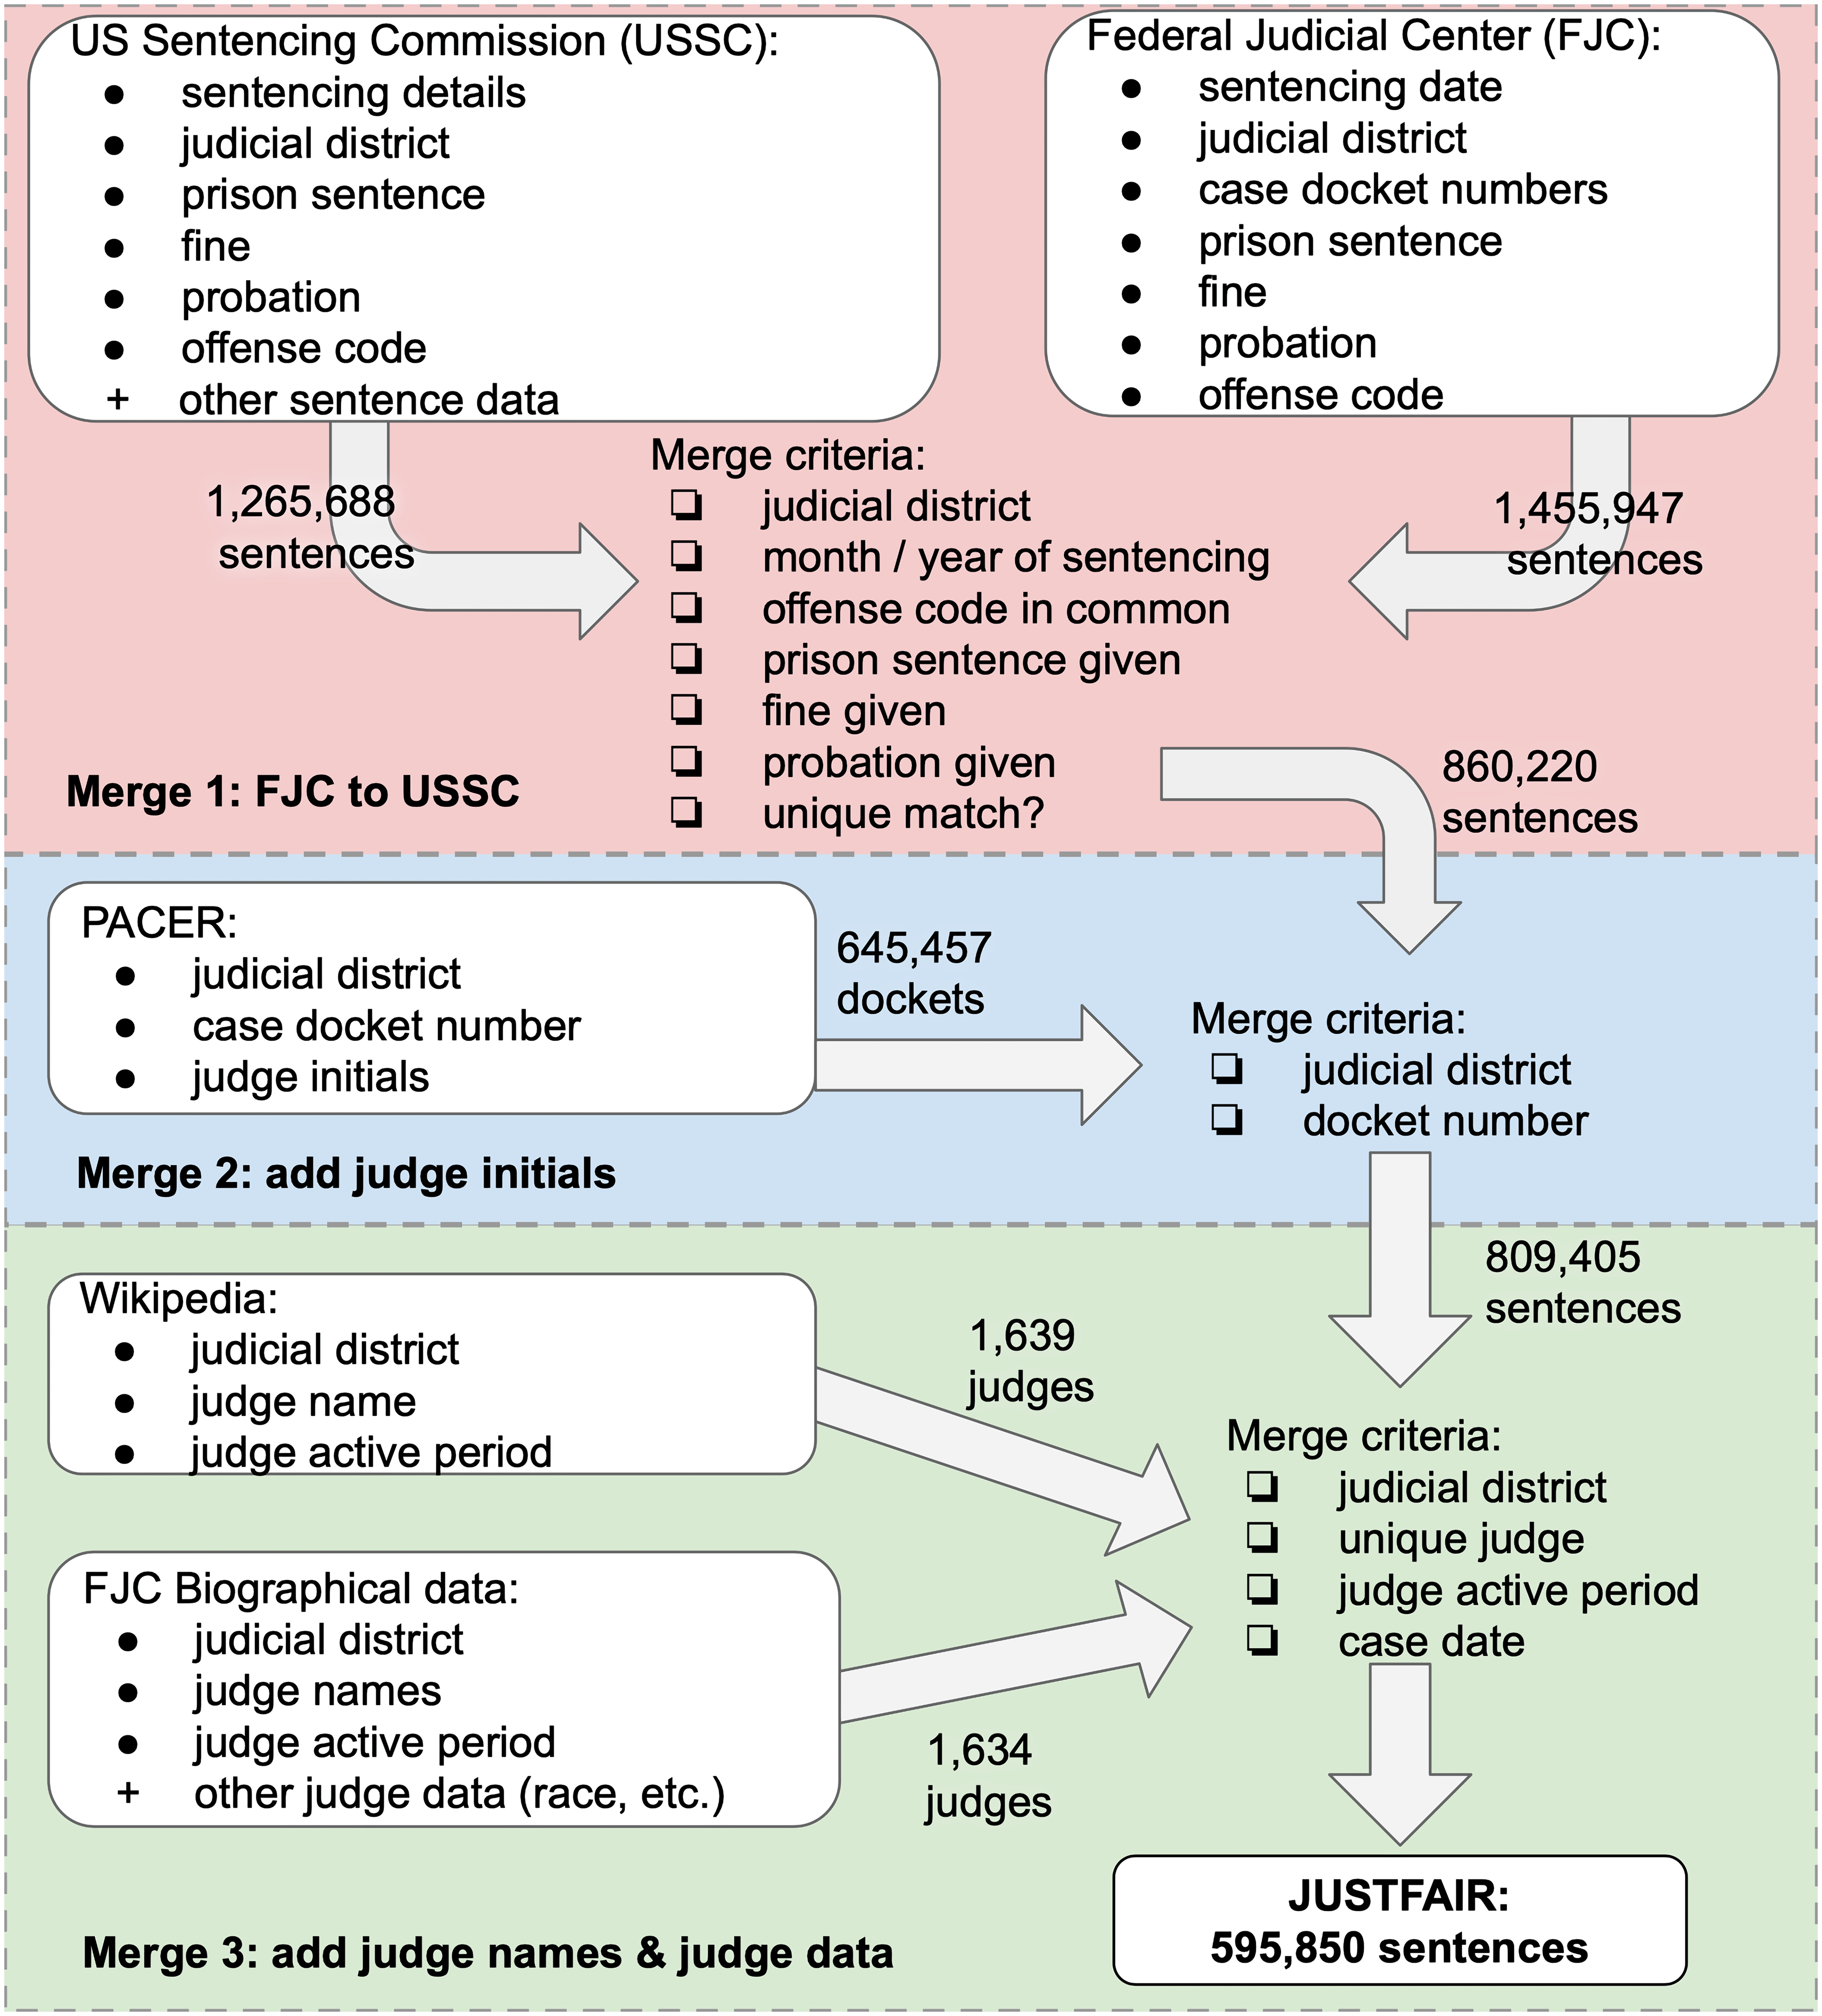
\includegraphics[width=\columnwidth]{Datasheets/JUSTFAIR_images/pone.0241381.g001.png}
    \caption{An illustration of how the five datasets are linked together to form the JUSTFAIR dataset. Reprinted from \cite{ciocanel2020justfair}.}
    \label{fig:link}
\end{figure}

Broadly, the information contains in the dataset consists of:

\begin{itemize}
    \item Sentencing Details
    \item Prison sentence
    \item Fine
    \item Probation
    \item Offense
    \item Judicial District
    \item Judge Name
    \item Defendant demographics
    \item Judge demographics
\end{itemize}

\subsection{Is there a target label or associated with each instance? \subtitle{Please include labels that are likely to be used as target labels, e.g. recidivism.}}

No. However, different aspects of sentencing, may be suitable to be used as target labels. 

\subsection{Are there recommended data splits (e.g., training, development/validation, testing)? \subtitle{If so, please provide a description of these splits, explaining the rationale behind them.}}

No.

\subsection{Does the dataset contain data on race and ethnicity? \subtitle{If so, is it based on the individual's self-description, or based on officer's impression? Was it collected or derived in post-processing? For example, by name analysis.}}

Yes. The dataset contains defendant demographic information, as well as demographic information on the judge .

\subsection{Are there any known errors, sources of noise, bias or missing data, or variables collected for only part of the datasets? \subtitle{If so, please provide a description.}}

JUSTFAIR uses a combination of Wikipedia and Federal Judicial Center biographical data to match the judge to the sentencing details. Based on 159 manual test cases, this matching has 2\% error rate.

\subsection{Does the dataset contain data on criminal history or other data that might be considered confidential or sensitive in any way? \subtitle{For example: sexual orientations, religious beliefs, political opinions or union memberships, or locations; financial or health data; biometric or genetic data; forms of government identification, such as social security numbers; If so, please provide a description.}}

The dataset contains sentencing data on individuals which may be considered confidential. 

\subsection{Is it possible to identify individuals (i.e., one or more natural persons), either directly or indirectly (i.e., in combination with other data) from the dataset? \subtitle{If so, please describe how.}}

Yes, the dataset purposely identifies the judges involved in the cases. In addition, the defendant's name also appears in the data.

\section{Uses}

\subsection{What type of tasks, if any, has the dataset been used for? \subtitle{If so, please provide examples and include citations.}}

The dataset has been used to study racial bias in the judicial system \cite{ciocanel2020justfair, smith2021most, sargent2021identifying, meyer2022flipping}.

\subsection{Is there a repository that links to any or all papers or systems that use the dataset? \subtitle{If so, please provide a link or other access point. }}

No.

\subsection{What (other) tasks could the dataset be used for? \subtitle{For example: testing predictive policing systems, predicting recidivism.}}

This dataset could be used to study research questions around sentencing and probation in the relevant courts. 


\subsection{Is there anything about the composition of the dataset or the way it was collected and preprocessed/cleaned/labeled that might impact future uses? \subtitle{For example, is there anything that a dataset consumer might need to know to avoid uses that could result in unfair treatment of individuals or groups (e.g., stereotyping, quality of service issues) or other risks or harms (e.g., legal risks, financial harms)? If so, please provide a description. Is there anything a dataset consumer could do to mitigate these risks or harms?}}

Results will have to be analyzed carefully due to the non-negligible error rate in judge-case matching. 

\section{Collection Process}

\subsection{How was the data associated with each instance acquired? \subtitle {e.g. the data collected survey, the raw data is routinely collected by the courts.}}

The dataset was created by merging five datasets:

\begin{enumerate}
    \item the United States Sentencing Commission Database
    \item the Federal Judicial Center Integrated Database
    \item the Public Access to Court Electronic Records system
    \item Wikipedia
    \item the Federal Judicial Center Biographical Directory of Article III Federal Judges
\end{enumerate}

\subsection{Was the information self-reported? \subtitle{If the data was self-reported, was the data validated/verified? If so, please describe how.}}

No. However, some of the information in the individual datasets, e.g., Wikipedia, may be self-reported.

\subsection{Who was involved in the data collection process? \subtitle{Was this done as part of their other duties? If not, were they compensated?}}

The data was collated by the QSIDE institute. 

\subsection{Over what timeframe was the data collected? Does this timeframe match the creation timeframe of the data associated with the instances (e.g., recent crawl of old news articles)? \subtitle{If not, please describe the timeframe in which the data associated with the instances was created. If the collection was not continuous within the timeframe, please specify the intervals, for example, annually, every 4 years, irregularly.}}

The dataset was published October 26, 2020, and covers the years 2001 –- 2018.

\subsection{Were any ethical review processes conducted (e.g., by an institutional review board)? \subtitle{If so, please provide a description of these review processes, including the outcomes, as well as a link or other access point to any supporting documentation.}}

An ethical review is not mentioned by the authors \cite{ciocanel2020justfair}.

\subsection{Were the individuals in question notified about the data collection? Did they give their consent? \subtitle{If consent was obtained, were the consenting individuals provided with a mechanism to revoke their consent in the future or for certain uses?}}

No.

\subsection{Has an analysis of the potential impact of the dataset and its use on data subjects (e.g., a data protection impact analysis) been conducted? \subtitle{If so, please provide a description of this analysis, including the outcomes, as well as a link or other access point to any supporting documentation.}}

An impact analysis is not mentioned by the authors \cite{ciocanel2020justfair}.

\section{Pre-processing, cleaning, labeling}

\subsection{Was any preprocessing/cleaning/labeling of the data done (e.g., discretization or bucketing, removal of instances, processing of missing values)? \subtitle{If so, please provide a description and reference to the documentation. If not, you may skip the remaining questions in this section.}}

The pre-processing performed on each of the five datasets can be found in \cite{ciocanel2020justfair}.

\subsection{Was the “raw” data saved in addition to the preprocessed/cleaned/labeled data? \subtitle{If so, please provide a link or other access point to the “raw” data. }}

The raw data is available on the respective websites of each of five datasets.

\subsection{Is the software that was used to preprocess/clean/label the data available? \subtitle{If so, please provide a link or other access point.}}

No.

\section{Distribution}

\subsection{Is the data publicly available? How and where can it be accessed (e.g., website, GitHub)? \subtitle{Does the dataset have a digital object identifier (DOI)?}}

Yes, the dataset can be downloaded at: \\ \href{https://qsideinstitute.org/research/criminal-justice/justfair/}{https://qsideinstitute.org/research/criminal-justice/justfair/}

\subsection{Is the dataset be distributed under a copyright or other intellectual property (IP) license, and/or under applicable terms of use (ToU)? \subtitle{If so, please describe this license and/or ToU, and provide a link or other access point to, or otherwise reproduce, any relevant licensing terms or ToU, as well as any fees associated with these restrictions.}}

No license has been specified.

\section{Maintenance}

\subsection{Is the dataset maintained? Who is supporting/hosting/maintaining the dataset?}

The dataset will be updated, conditional on the creators obtaining additional funding.

\subsection{How can the owner/curator/manager of the dataset be contacted (e.g., email address)?}

The QSIDE Institute can be contacted at: qside@qsideinstitute.org

\subsection{Will the dataset be updated (e.g., to correct labeling errors, add new instances, delete instances)?}

Yes, conditional on the creators obtaining additional funding.

\subsection{Are older versions of the dataset continue to be supported/hosted/maintained?}

No.

\subsection{If others want to extend/augment/build on/contribute to the dataset, is there a mechanism for them to do so? \subtitle{If so, please provide a description.}}

Try contacting qside@qsideinstitute.org.


\medskip
 
\bibliographystyle{unsrt}  
\bibliography{JUSTFAIR_datasheet}

\end{document}
